\documentclass[9pt]{article}

\usepackage{amsmath}
\usepackage{tcolorbox}
% `parskip` removes indentation for all paragraphs: http://tex.stackexchange.com/a/55016
\usepackage{parskip}
% Allows us to color rows / cols of a table.
% See https://texblog.org/2011/04/19/highlight-table-rowscolumns-with-color/
\usepackage{color, colortbl}

\usepackage{hyperref}
\graphicspath{{images/ps7/}}

\leftmargin=0.25in
\oddsidemargin=0.25in
\textwidth=6.0in
\topmargin=-0.25in
\textheight=9.25in

\definecolor{Gray}{gray}{0.9}

\begin{document}

\begin{center}
  \large\textbf{MIT 18.01 Problem Set 7 Unofficial Solutions}
\end{center}

\begin{tcolorbox}
  \textbf{Q1)} (from PS6) The voltage $V$ of house current is given by\\
  \begin{center}
    $V(t) = Csin(120\pi t)$
  \end{center}
  \begin{center}
  \end{center}
  where $t$ is time, in seconds and $C$ is a constant amplitude. The square root of the average value of $V^2$ over one period of $V(t)$ (or cycle) is called the \emph{root-mean-square} voltage, abbreviated RMS. This is what the voltage meter on a house records. For house current, find the RMS in terms of the constant $C$. (The peak voltage delivered to the house is $\pm C$. The units of $V^2$ are square volts; when we take the square root again after averaging, the units become volts again.)
\end{tcolorbox}

Average value of $V^2$ over $1$ period of $V(t)$ is

\begin{align*}
  \frac{1}{60} \int_0^{\frac{1}{60}} C^2 sin^2(120\pi t) dt &= \frac{C^2}{60} \int_0^{\frac{1}{60}} sin^2(120\pi t) dt \\
  &= \frac{C^2}{60} \int_0^{\frac{1}{60}} \frac{1 - cos(240\pi t)}{2} dt \\
  &= \frac{C^2}{120} \int_0^{\frac{1}{60}} 1 - cos(240\pi t) dt \\
  &= \frac{C^2}{120} (t - \frac{sin(240\pi t)}{240\pi}) \bigg]_0^{\frac{1}{60}} \\
  &= \frac{C^2}{120} (\frac{1}{60} - \frac{sin(240\pi \cdot \frac{1}{60})}{240\pi}) \\
  &= \frac{C^2}{120} (\frac{1}{60} - \frac{sin(4\pi)}{240\pi}) \\
  &= \frac{C^2}{120} (\frac{1}{60}) \\
  &= \frac{C^2}{7200}
\end{align*}

Square root of average value of $V^2$ over 1 period of $V(t) = \sqrt{\frac{C^2}{7200}} = \frac{C}{\sqrt{3600 * 2}} = \frac{C}{60\sqrt{2}}$


\begin{tcolorbox}
  \textbf{Q2)} The solid torus is the figure obtained by rotating the disk $(x - b)^2 + y^2 \leq a^2$ around the $y$-axis. Find its volume by the method of shells. (Hint: Substitute for $x - b$. As noted p. 229/11, the answer happens to be the area of the disk multiplied by the distance travelled by the center as it revolves.)
\end{tcolorbox}

\begin{center}
  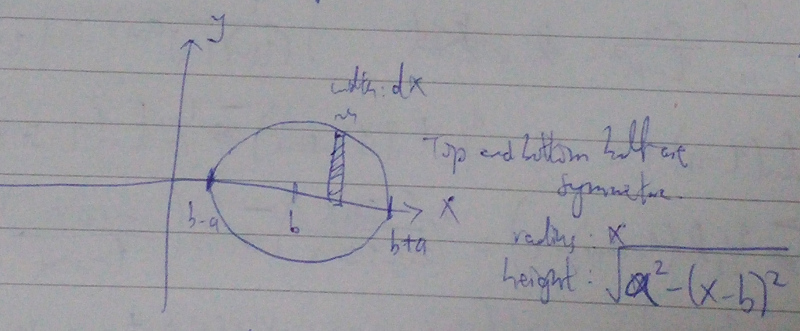
\includegraphics[scale=0.5]{q2.jpg}
\end{center}

For a circle centered at $x = b, y = 0$ with radius $a$, the volume of the torus is:

\begin{align*}
  2 \int_{b-a}^{b+a} 2 \pi x (\sqrt{a^2 - (x - b)^2}) dx &= 4 \pi \int_{b-a}^{b+a} x \sqrt{a^2 - (x - b)^2} dx
\end{align*}

Let $u = x - b$. Then $du = dx$. Also, $x = u + b$. Substitute those into the above:

\begin{align*}
  4 \pi \int_{b-a}^{b+a} x \sqrt{a^2 - (x - b)^2} dx &= 4 \pi \int_{-a}^{a} (u + b) \sqrt{a^2 - u^2} du \\
  &= 4 \pi (\int_{-a}^{a} u \sqrt{a^2 - u^2} du + b \int_{-a}^{a} \sqrt{a^2 - u^2} du) \\
  &= 4\pi ( -\frac{1}{2} \cdot \frac{({a^2 - u^2})^{3/2}}{\frac{3}{2}} \bigg]_{-a}^{a} + b \int_{-a}^{a} \sqrt{a^2 - u^2} du ) \\
  &= 4 \pi b \int_{-a}^{a} \sqrt{a^2 - u^2} du \ \ \ \ \text{(area of semicircle of radius $a$ centered at origin)} \\
  &= 4 \pi b (\frac{1}{2} \pi a^2) \\
  &= 2 \pi^2 a^2 b
\end{align*}

\end{document}
